\documentclass{article}
\usepackage[utf8]{inputenc}
\usepackage{float}
\usepackage{lastpage}
\usepackage{graphicx}
\usepackage[margin=1.1in]{geometry}
\usepackage{listings} 
\usepackage{watermark}
\usepackage{blindtext}
\usepackage{amsmath}
\usepackage{float}
\usepackage{footnote}
\usepackage{multirow}
\makesavenoteenv{table}
%\usepackage[svgnames]{xcolor}
\usepackage{subfig}
\usepackage{hyperref}
\usepackage{xcolor}
\usepackage{booktabs} % To thicken table lines
\usepackage{amsmath}
\usepackage{mathtools}
\newcommand{\link}[1]{{\color{blue}\href{#1}{#1}}}
\usepackage[justification=centering]{caption}
\usepackage[section]{placeins}
\usepackage{fancyhdr}
\pagestyle{fancy}
\lhead{Final Project}
\rhead{10339 Concepts in Heterogeneous Catalysis}
\linespread{1.3} % Line spacing
%\setlength\parindent{0pt} % Uncomment to remove all indentation from paragraphs
\usepackage{geometry}
 \geometry{
 a4paper,
 total={170mm,257mm},
 left=22mm,
 right=22mm,
 top=30mm,
 bottom=20mm
 }
 
 
 
\begin{document}

% the first title page
%\renewcommand{\headrulewidth}{0.4pt} %header
\cfoot{\thepage\ of \pageref{LastPage}}
%-------------------------------------------------------------------------------
%	TITLE PAGE
%-------------------------------------------------------------------------------
\begin{titlepage}
\newcommand{\HRule}{\rule{\linewidth}{0.5mm}} % Defines a new command for the horizontal lines, change thickness here
\center % Center everything on the page

\includegraphics[width=0.15\textwidth]{Pictures/DTU-logo.pdf}
\\[0.5cm]
% \textsc{\large \textbf{02901 Advanced Topics in Machine Learning}:\\ Latest developments in machine learning at {\it ICML 2021} }\\[0.5cm] % Minor heading such as course title
\HRule \\[0.8cm]
{ \huge \bfseries Final Project in 10339 Concepts in Heterogeneous Catalysis, Autumn 2021\\[0.4cm] % Title of your document
\HRule \\[3cm]
\begin{minipage}{0.8\textwidth}
\begin{center} 
\emph{Student: Changzhi Ai} 
\end{center}
\end{minipage}\\[2cm]
{\large 
\today %dato 
}
\\[0.2cm] % Date, change the \today to a set date if you want to be precise
\thiswatermark{\centering \put(-180,-720){
\includegraphics[scale=0.6]{Pictures/DTU-frise-SH-15.pdf}} }
}\end{titlepage}



\newpage
\section{Introduction}
    We consider the dehydrogenation of CH4(g) into CH3* and H* and the association of C* and O* forming CO* as potential rate-limiting steps. It would be a catalyst if the difference of activation energy and reaction energy is not very high during these steps.

 
\section{Methods}
    \subsection*{Detail the strategies, tools, and equations you use.}
    We have 9 different elementary steps as the following: \\
    $$ 1.\;\; \text{CH}_4(g)+2\text{}^* \rightleftharpoons \text{CH}_3^* + \text{H}^* $$
    $$ 2.\;\;  \text{CH}_3^*+ \text{}^* \rightleftharpoons \text{CH}_2^* + \text{H}^* $$
    $$ 3.\;\;  \text{CH}_2^*+ \text{}^* \rightleftharpoons \text{CH}^* + \text{H}^* $$
    $$ 4.\;\; \text{CH}^*+ \text{}^* \rightleftharpoons \text{C}^* + \text{H}^* $$
    $$ 5.\;\;  \text{H}_2\text{O}(g)+2\text{}^* \rightleftharpoons \text{OH}^* + \text{H}^* $$
    $$ 6.\;\; \text{OH}^*+\text{}^* \rightleftharpoons \text{O}^* + \text{H}^* $$
    $$ 7.\;\; \text{C}^*+ \text{O}^* \rightleftharpoons \text{CO}^* + \text{}^* $$
    $$ 8.\;\; \text{CO}^* \rightleftharpoons \text{CO}(g) + \text{}^* $$
    $$ 9.\;\; \text{H}^*+\text{H}^* \rightleftharpoons \text{H}_2(g) + 2\text{}^* $$
    According the these elementary equations, we extract the reaction energies and activation energies of different surfaces. Their reaction energies and activation energies of Ag(211), Au(211), Cu(211) and Pt(211) surfaces in all 9 steps can be directly obtained from catapp, but their energies of Ru(211) and Rh(211) in step 9 are not in the database of catapp. Therefore, I would first try to get potential energies and free energies in each step using Ag(211), Au(211), Cu(211) and Pt(211) surfaces. The rate constants and equilibrium constants could be calculated according to these energies after the partital pressure and temperature are provided. And then we can get kinetic activities of limiting step through solving kinetic equations. Therefore, the scaling relations of different intermediates could be also obtained according to potential energies and free energies in each step. After giving the descriptor of activities and scaling relations, we would get the final activity volcano. Then, if we know the value of the descriptor of Ru(211) and Rh(211), we would get their activity. 
    
    We have 11 species and 4 gas (actually more species if including transition state species):
    \begin{eqnarray}
        E_{CH_{4}} =& 0 \nonumber \\
        E_{H_2} =& 0 \nonumber \\
        E_{H_{2}O} =& 0 \nonumber \\
        E_{CO} = \Delta E_{rxn} - 3 E_{H_{2}} + E_{CH_{4}} + E_{H_{2}O} =& 2.94 \nonumber \\
        E_{CH_3*} =& \Delta E_1 + \frac{1}{2}\Delta E_9 \nonumber \\
        E_{CH_2*} =& \Delta E_1 + \Delta E_2  + \Delta E_9 \nonumber \\
        E_{CH*} =& \Delta E_1 + \Delta E_2 + \Delta E_3 + \frac{3}{2}\Delta E_9 \nonumber \\
        E_{C*} =& \Delta E_1 + \Delta E_2 + \Delta E_3 + \Delta E_4 + 2\Delta E_9 \nonumber
    \end{eqnarray}
    \begin{eqnarray}
        E_{OH*} =& \Delta E_5 + \frac{1}{2}\Delta E_9 \nonumber \\
        E_{O*} =& \Delta E_5 + \Delta E_6 + \Delta E_9 \nonumber \\
        E_{CO*} =& E_{CO} - \Delta E_8 \nonumber \\
        E_{H*} =& - \frac{1}{2}\Delta E_9 \nonumber \\
        E_{CH_{3}-H*} =& \Delta E_{a,1} \nonumber \\
        E_{C-O*} =& \Delta E_{a,7} + E_{CO} - \Delta E_7 - \Delta E_8 \nonumber
    \end{eqnarray}
    \subsection*{State the assumptions you make and justify them appropriately.}
    The quasi-equilibriated reactions 2, 3, 4, 5, 6, 8 and 9 give:
\begin{eqnarray}
    \theta_{CH_{3}}= \frac{\theta_{C} P_{H_2}^{\frac{3}{2}}}{K_{2} K_{3} K_{4} K_{9}^{\frac{3}{2}}}  \\
    \theta_{CH_{2}}= \frac{\theta_{C} P_{H_2}}{K_{3} K_{4} K_{9}}   \\
    \theta_{CH}= \frac{\theta_{C} P_{H_2}^{\frac{1}{2}}}{K_{4} K_{9}^{\frac{1}{2}}}   \\
    \theta_{O}= \frac{K_{5} K_{6} K_{9} \theta_{*} P_{H_{2}O}}{P_{H_2}}   \\
    \theta_{OH}= \frac{K_{5} K_{9}^{\frac{1}{2}} \theta_{*} P_{H_{2}O}}{P_{H_2}^\frac{1}{2}}   \\
    \theta_{CO}= \frac{P_{CO} \theta_{*}}{K_{8}}   \\
    \theta_{H}= \frac{P_{H_2}^{\frac{1}{2}} \theta_{*}}{K_{9}^\frac{1}{2}}
\end{eqnarray}

If step 1 is limiting:
% \FloatBarrier
% \begin{figure}[!ht]
%     \centering
%     % \includegraphics[width=0.25\textwidth]{mesh}
%     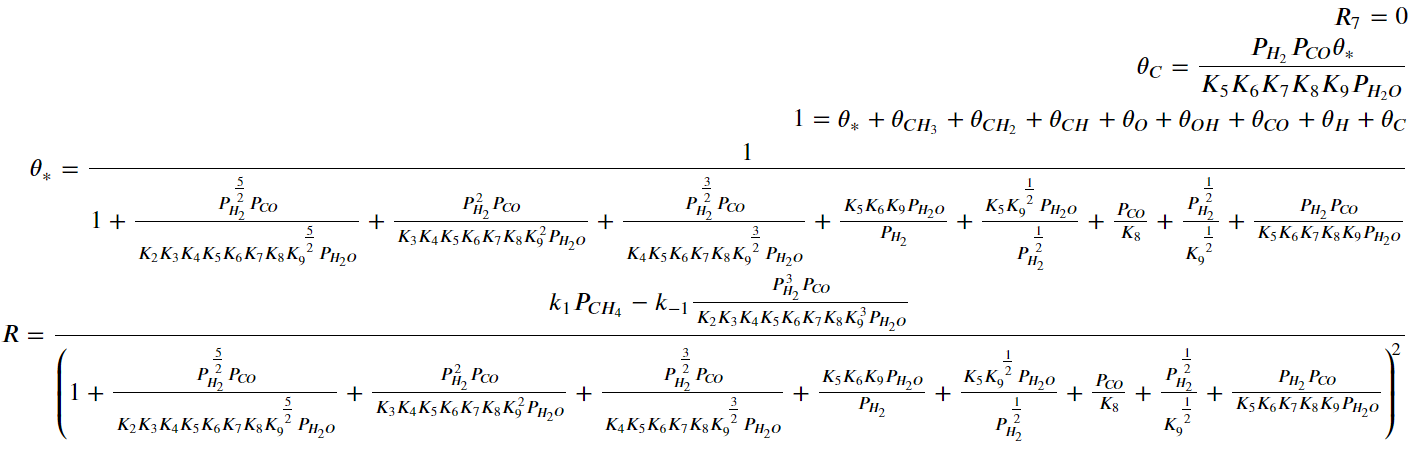
\includegraphics[width=1\textwidth]{Pictures/R1.png}
%     \caption{}
%     \label{fig:R1}
% \end{figure}

\begin{eqnarray}
    R_{7} = 0  \\
    \theta_{C}= \frac{P_{H_2} P_{CO} \theta_{*}}{K_{5} K_{6} K_{7} K_{8} K_{9} P_{H_{2}O}} \nonumber  \\
    1 = \theta_{*}+\theta_{CH_{3}}+\theta_{CH_{2}}+\theta_{CH}+\theta_{O}+\theta_{OH}+\theta_{CO}+\theta_{H}+\theta_{C}
\end{eqnarray}
\begin{eqnarray}
    \theta_* = \frac{1}
    {
    \begin{multlined}
    1 + \frac{P_{H_2}^{\frac{5}{2}} P_{CO}}{K_{2} K_{3} K_{4} K_{5} K_{6} K_{7} K_{8} K_{9}^{\frac{5}{2}} P_{H_{2}O}} + \frac{P_{H_2}^2 P_{CO}}{K_{3} K_{4} K_{5} K_{6} K_{7} K_{8} K_{9}^2 P_{H_{2}O}} + \frac{P_{H_2}^{\frac{3}{2}} P_{CO}}{K_{4} K_{5} K_{6} K_{7} K_{8} K_{9}^{\frac{3}{2}} P_{H_{2}O}} + \\ \frac{K_{5} K_{6} K_{9} P_{H_{2}O}}{P_{H_2}} + \frac{K_{5} K_{9}^{\frac{1}{2}} P_{H_{2}O}}{P_{H_2}^\frac{1}{2}} +  \frac{P_{CO}}{K_{8}} + \frac{P_{H_2}^{\frac{1}{2}}}{K_{9}^\frac{1}{2}} + \frac{P_{H_2} P_{CO}}{K_{5} K_{6} K_{7} K_{8} K_{9} P_{H_{2}O}}
    \end{multlined}
    }  \\
    R = \frac{ k_{1}P_{CH_{4}} - k_{-1} \frac{P_{H_2}^{3} P_{CO}}{K_{2} K_{3} K_{4} K_{5} K_{6} K_{7} K_{8} K_{9}^{3} P_{H_{2}O}} }  
    {\left({
    \begin{multlined}
     1 + \frac{P_{H_2}^{\frac{5}{2}} P_{CO}}{K_{2} K_{3} K_{4} K_{5} K_{6} K_{7} K_{8} K_{9}^{\frac{5}{2}} P_{H_{2}O}} + \frac{P_{H_2}^2 P_{CO}}{K_{3} K_{4} K_{5} K_{6} K_{7} K_{8} K_{9}^2 P_{H_{2}O}} + \frac{P_{H_2}^{\frac{3}{2}} P_{CO}}{K_{4} K_{5} K_{6} K_{7} K_{8} K_{9}^{\frac{3}{2}} P_{H_{2}O}} + \\
    \frac{K_{5} K_{6} K_{9} P_{H_{2}O}}{P_{H_2}} + \frac{K_{5} K_{9}^{\frac{1}{2}} P_{H_{2}O}}{P_{H_2}^\frac{1}{2}} + \frac{P_{CO}}{K_{8}} + \frac{P_{H_2}^{\frac{1}{2}}}{K_{9}^\frac{1}{2}} + \frac{P_{H_2} P_{CO}}{K_{5} K_{6} K_{7} K_{8} K_{9} P_{H_{2}O}} 
    \end{multlined}
    }\right) ^2} 
\end{eqnarray}


If step 7 is limiting:
\begin{eqnarray}
    R_{1} = 0  \\
    \theta_{C}= \frac{K_{1} K_{2} K_{3} K_{4} K_{9}^2 P_{CH_4} \theta_{*}}{P_{H_2}^2}  \\
    1 = \theta_{*}+\theta_{CH_{3}}+\theta_{CH_{2}}+\theta_{CH}+\theta_{O}+\theta_{OH}+\theta_{CO}+\theta_{H}+\theta_{C} \\
    \theta_* = \frac{1}
    {
    \begin{multlined}
    1 + \frac{K_{1} P_{CH_4} K_{9}^{\frac{1}{2}}}{P_{H_2}^{\frac{1}{2}}} + \frac{K_{1} K_{2} K_{9} P_{CH_4}}{P_{H_2}} + \frac{K_{1} K_{2} K_{3} K_{9}^{\frac{3}{2}} P_{CH_4}}{P_{H_2}^{\frac{3}{2}}} + \frac{K_{5} K_{6} K_{9} P_{H_{2}O}}{P_{H_2}} + \\ \frac{K_{5} K_{9}^{\frac{1}{2}} P_{H_{2}O}}{P_{H_2}^\frac{1}{2}} + \frac{P_{CO}}{K_{8}} + \frac{P_{H_2}^{\frac{1}{2}}}{K_{9}^\frac{1}{2}} + \frac{K_{1} K_{2} K_{3} K_{4} K_{9}^2 P_{CH_4}}{P_{H_2}^2}
    \end{multlined}
    } \\
    R = \frac{ k_{7} \frac{K_{1} K_{2} K_{3} K_{4} K_{5} K_{6} K_{9}^3 P_{CH_4} P_{H_{2}O}}{P_{H_2}^3} - k_{-7} \frac{P_{CO}}{K_{8}} }  
    {\left({
    \begin{multlined}
    1 + \frac{K_{1} P_{CH_4} K_{9}^{\frac{1}{2}}}{P_{H_2}^{\frac{1}{2}}} + \frac{K_{1} K_{2} K_{9} P_{CH_4}}{P_{H_2}} + \frac{K_{1} K_{2} K_{3} K_{9}^{\frac{3}{2}} P_{CH_4}}{P_{H_2}^{\frac{3}{2}}} + \frac{K_{5} K_{6} K_{9} P_{H_{2}O}}{P_{H_2}} + \frac{K_{5} K_{9}^{\frac{1}{2}} P_{H_{2}O}}{P_{H_2}^\frac{1}{2}} + \frac{P_{CO}}{K_{8}} +\\ \frac{P_{H_2}^{\frac{1}{2}}}{K_{9}^\frac{1}{2}} + \frac{K_{1} K_{2} K_{3} K_{4} K_{9}^2 P_{CH_4}}{P_{H_2}^2}
    \end{multlined}
    } \right)^2 }
\end{eqnarray}

 
\section{Results}
    \subsection*{Potential/Free energy diagrams}
    Figure \ref{fig:Energy_diagram} shows potential energy diagram and free energy diagram, respectively. We have 9 elementary reactions and reaction 9 happens 3 times. 0.002 eV/K entropy corrections for gas are added during the calculation of free energies.
    \FloatBarrier
    \begin{figure}[!ht]
        \centering
        % \includegraphics[width=0.25\textwidth]{mesh}
        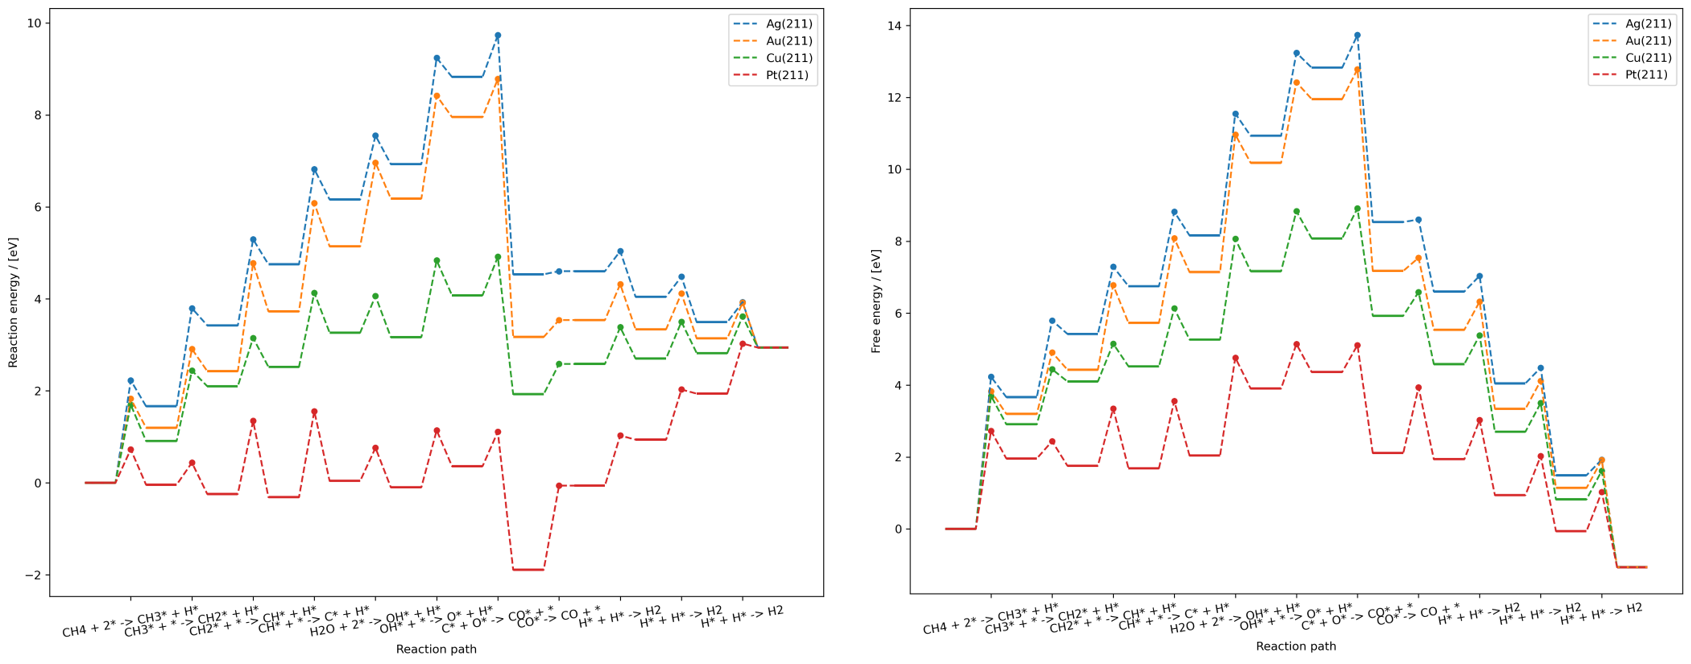
\includegraphics[width=1\textwidth]{Pictures/Energy_diagram.png}
        \caption{Potential and free energy diagrams of Ag(211), Au(211), Cu(211) and Pt(211) surfaces.}
        \label{fig:Energy_diagram}
    \end{figure}
    
    % \FloatBarrier
    % \begin{figure}[!ht]
    %     \centering
    %     % \includegraphics[width=0.25\textwidth]{mesh}
    %     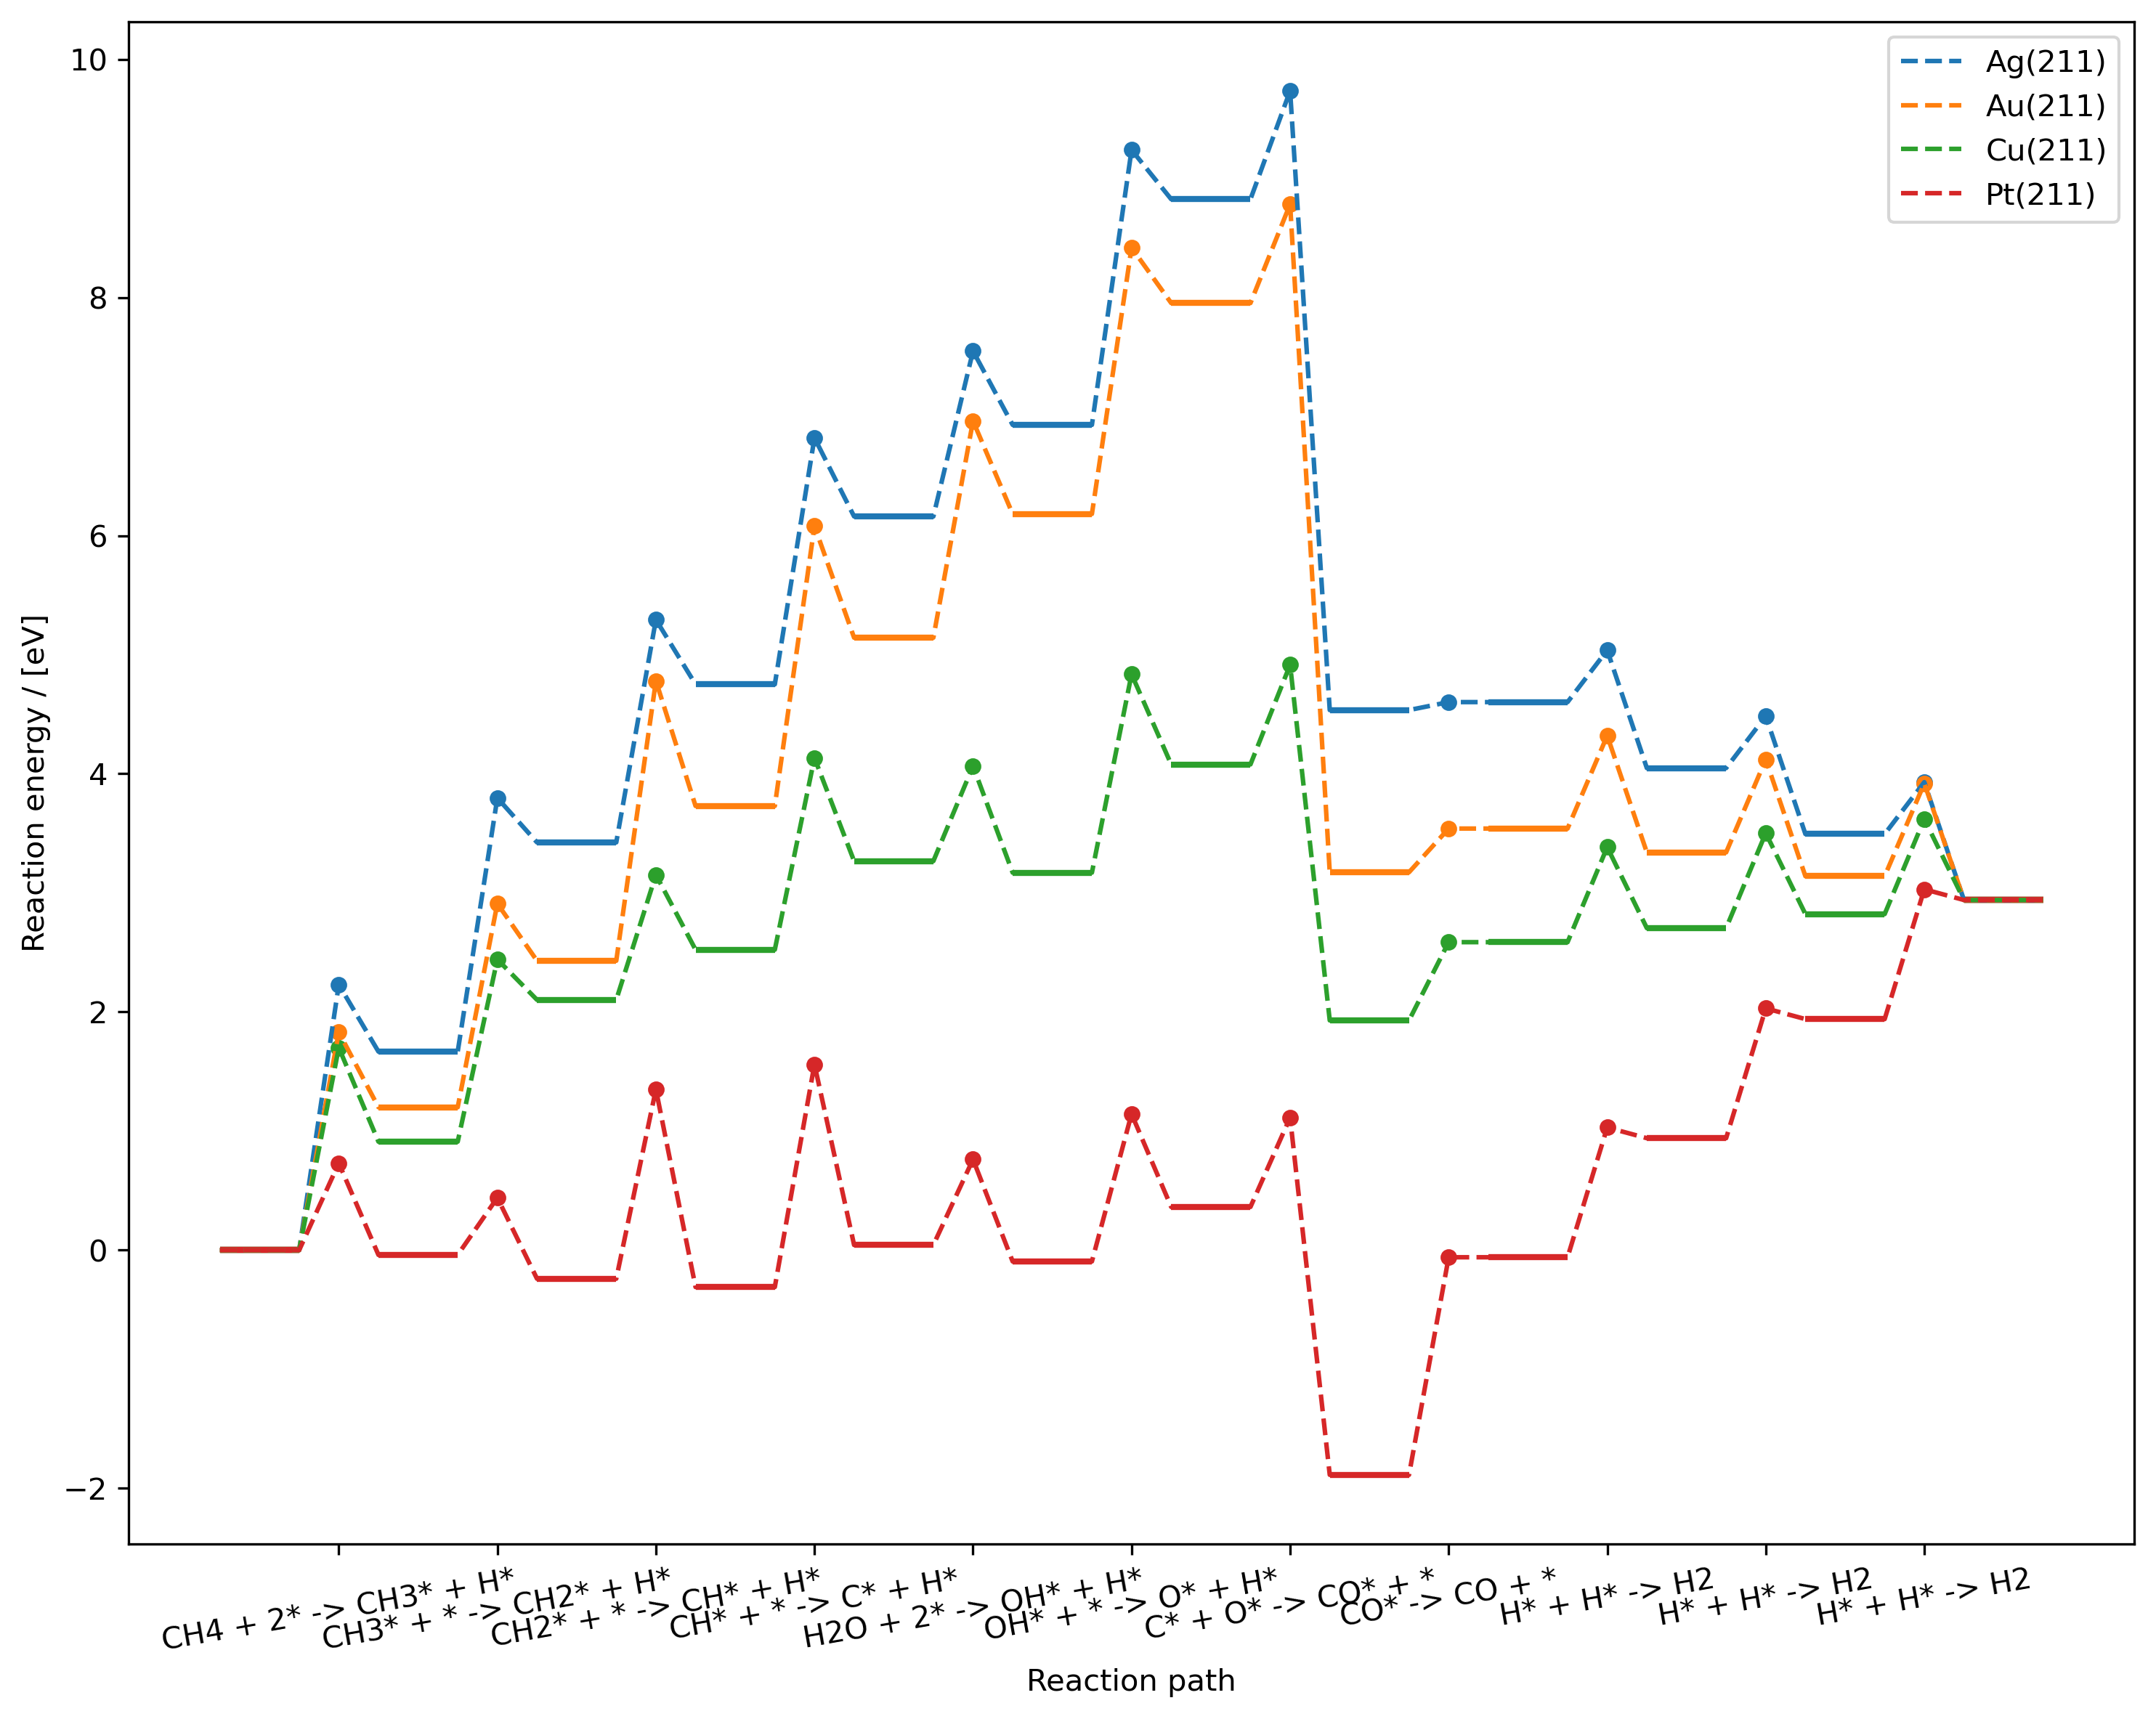
\includegraphics[width=0.7\textwidth]{Pictures/Reaction_energy.png}
    %     \caption{Potential and free energy diagrams of Ag(211), Au(211), Cu(211) and Pt(211) surfaces.}
    %     \label{fig:Potential_energy}
    % \end{figure}
    
    % \FloatBarrier
    % \begin{figure}[!ht]
    %     \centering
    %     % \includegraphics[width=0.25\textwidth]{mesh}
    %     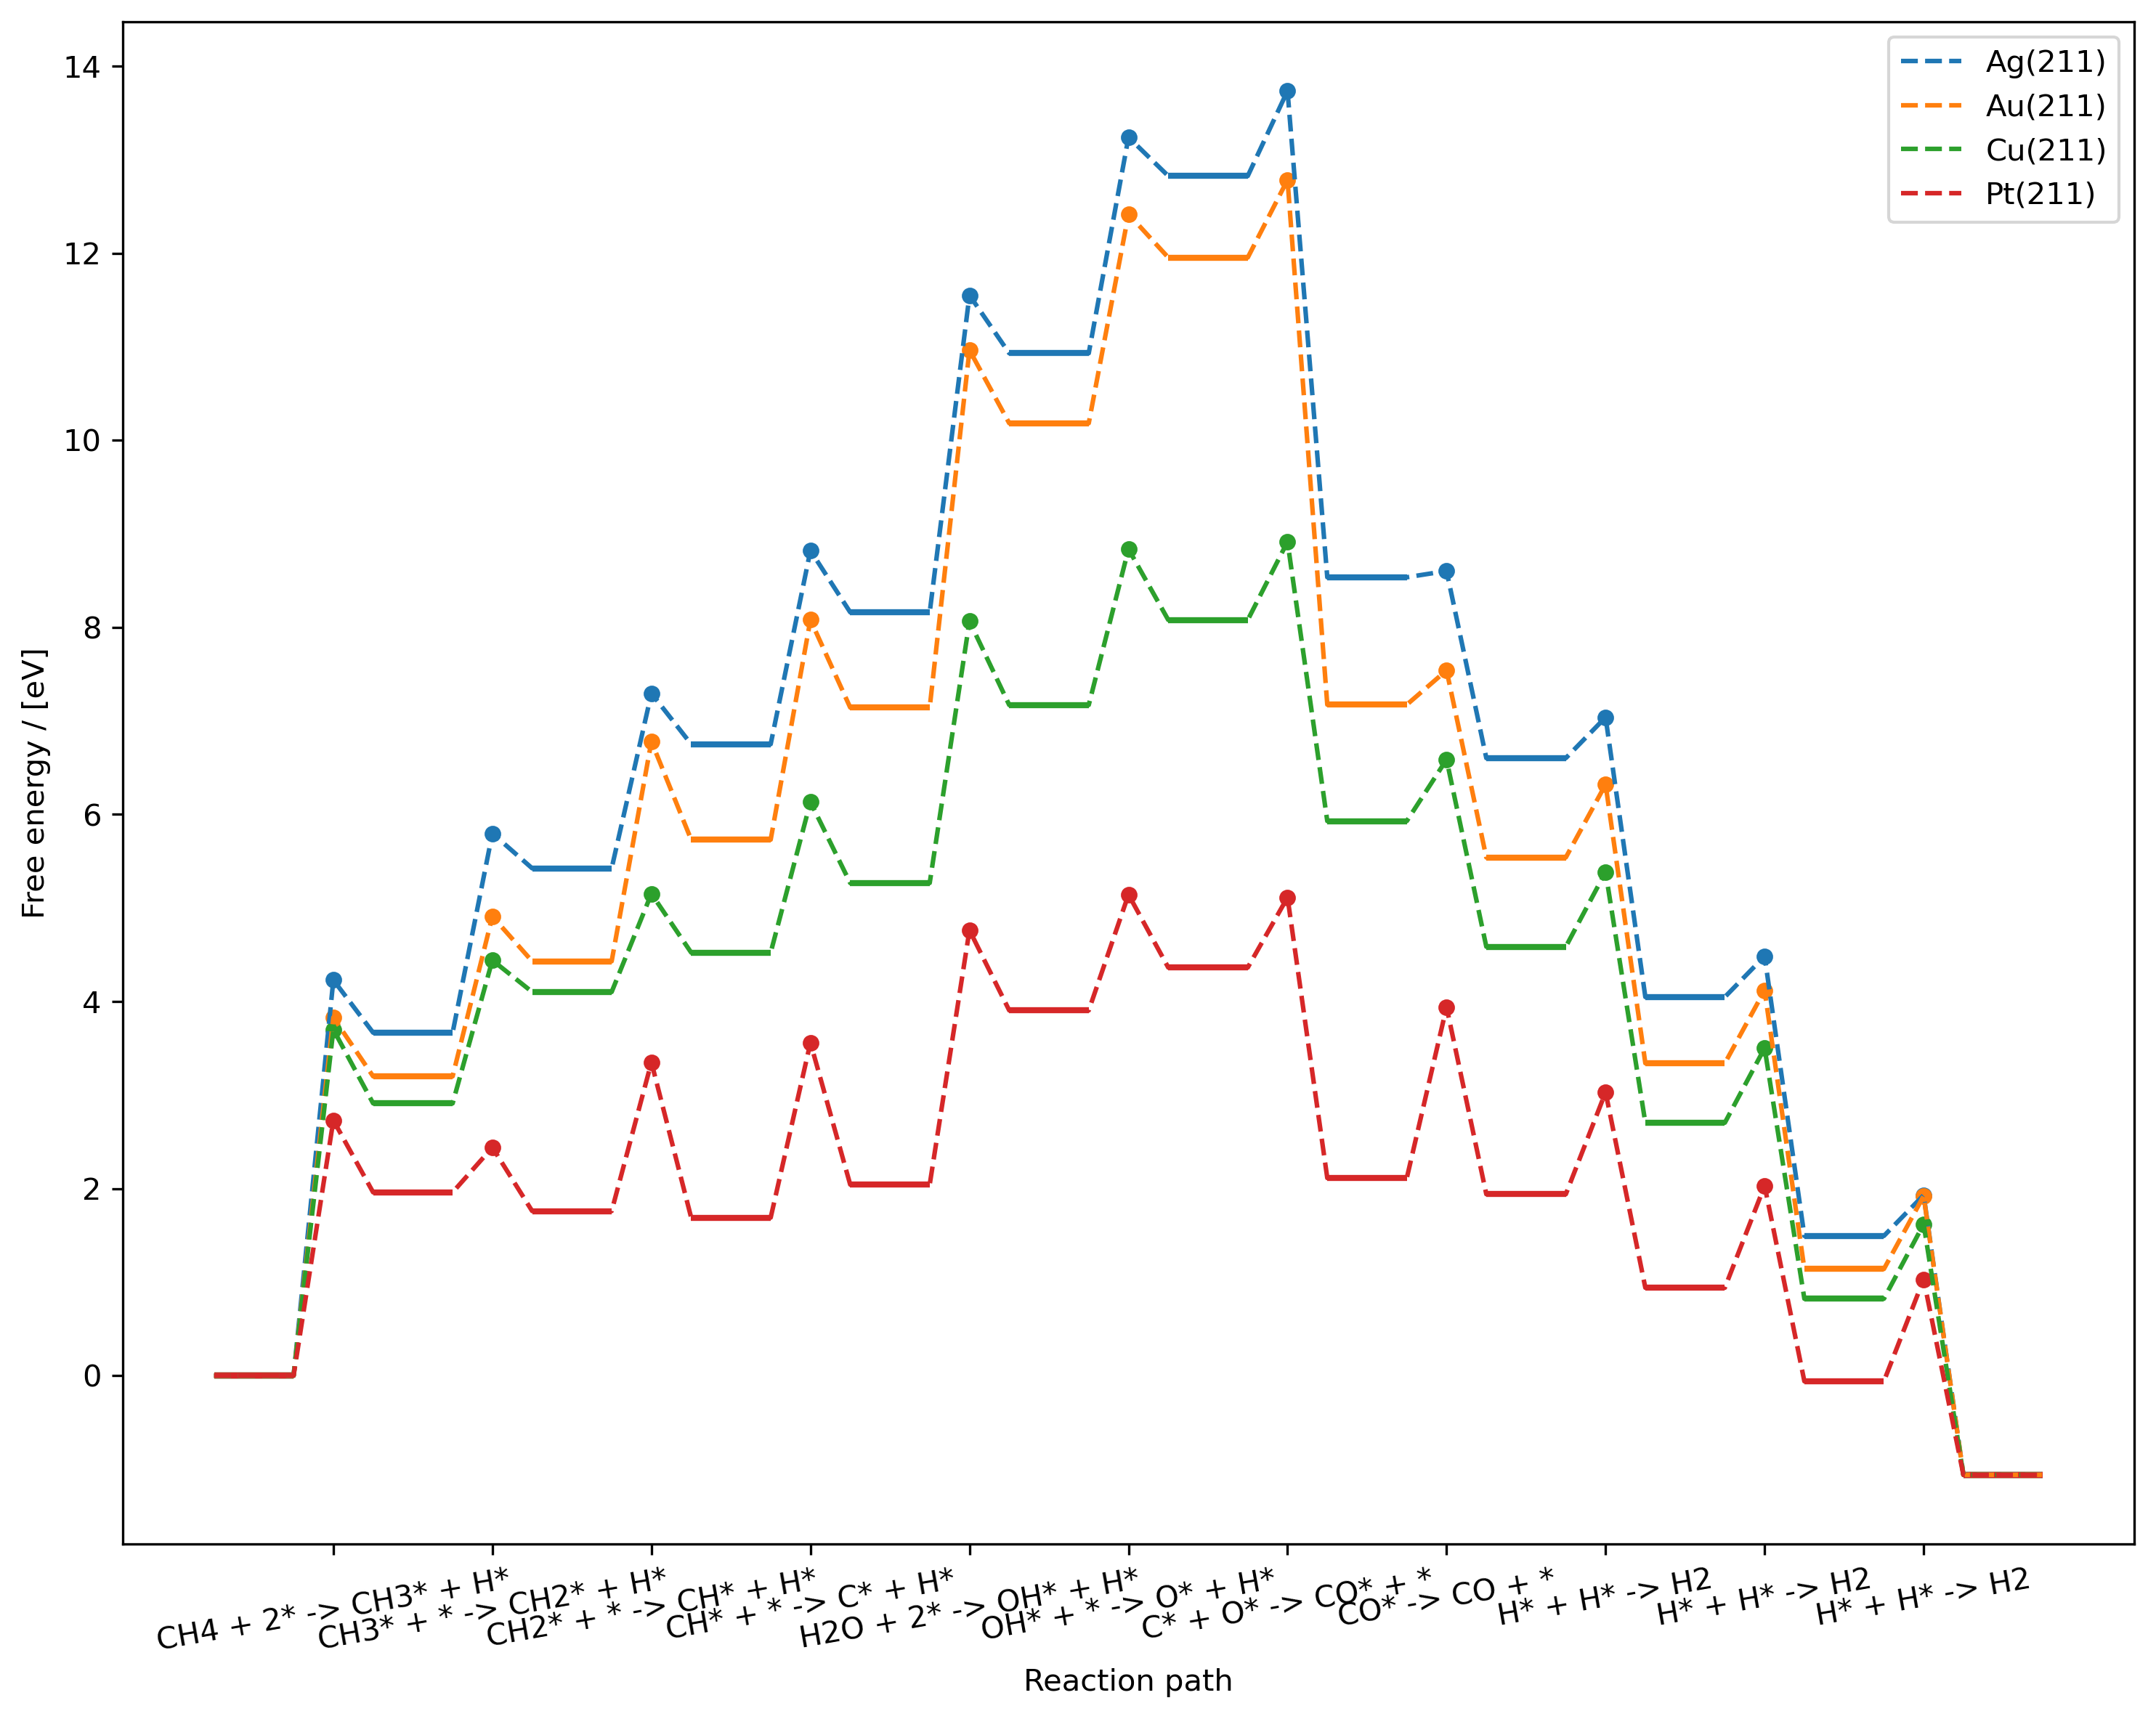
\includegraphics[width=0.7\textwidth]{Pictures/Free_energy.png}
    %     \caption{Free energy diagram of Ag(211), Au(211), Cu(211) and Pt(211) surfaces.}
    %     \label{fig:Free_energy}
    % \end{figure}

    
    \subsection*{Scaling relations}
    Figure \ref{fig:Scaling_relation} shows all scaling relations of Ag(211), Au(211), Cu(211) and Pt(211) surfaces between different intermediates and descriptor. We can see that there are really good scaling relations.
    \FloatBarrier
    \begin{figure}[!ht]
        \centering
        % \includegraphics[width=0.25\textwidth]{mesh}
        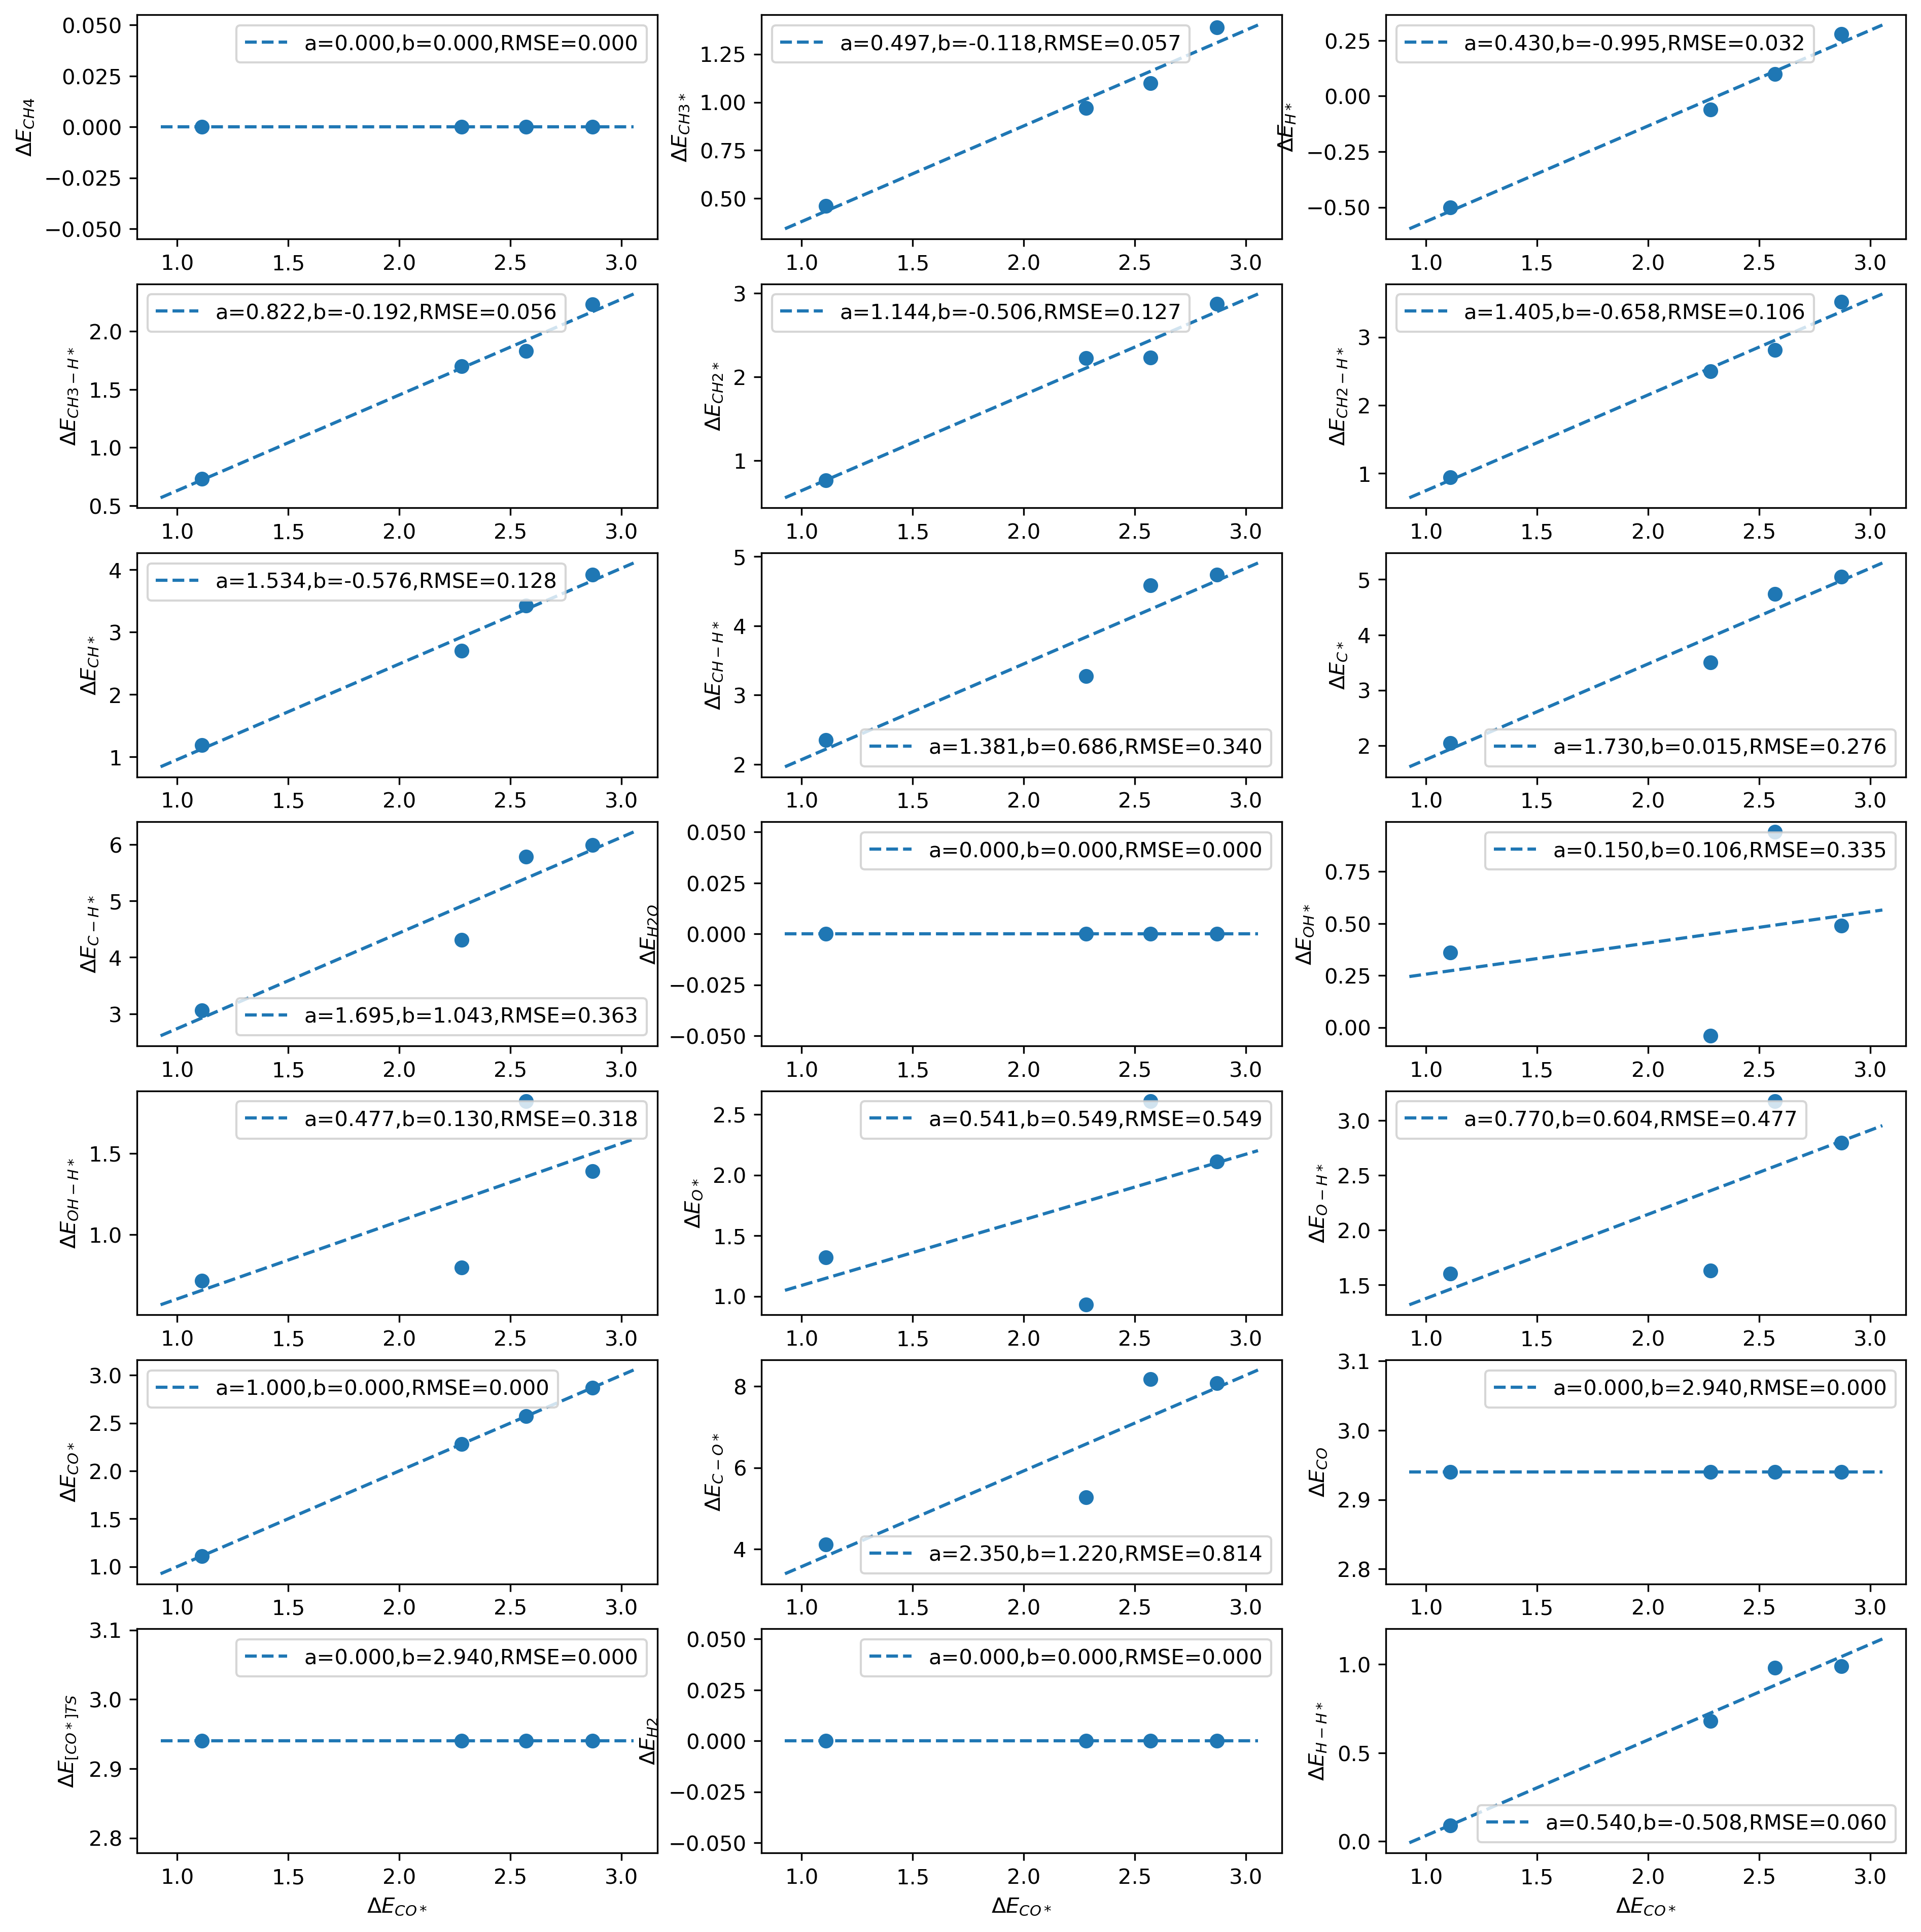
\includegraphics[width=0.9\textwidth]{Pictures/Scaling_relation.png}
        \caption{Scaling relations of Ag(211), Au(211), Cu(211) and Pt(211) surfaces between different intermediates and descriptor.}
        \label{fig:Scaling_relation}
    \end{figure}

    
    \subsection*{How the choice of the descriptors may affect the final results}
    The choice of the descriptors will influence how good the scaling relations are. And the scaling relations can the precision of activity volcano. Therefore, the choice of the descriptors would affect how good the kinetic model is. Here, it can be notice that there exist good scaling relations when the CO* descriptor is chosen.
    
    \subsection*{Kinetic calculations}
    Kinetic activities of Ag(211), Au(211), Cu(211) and Pt(211) surfaces are shown in Figure \ref{fig:Kinetic_calculation}. It can be noticed that Pt(211) has better kinetic performance compared to the other three surfaces.
    \FloatBarrier
    \begin{figure}[!ht]
        \centering
        % \includegraphics[width=0.25\textwidth]{mesh}
        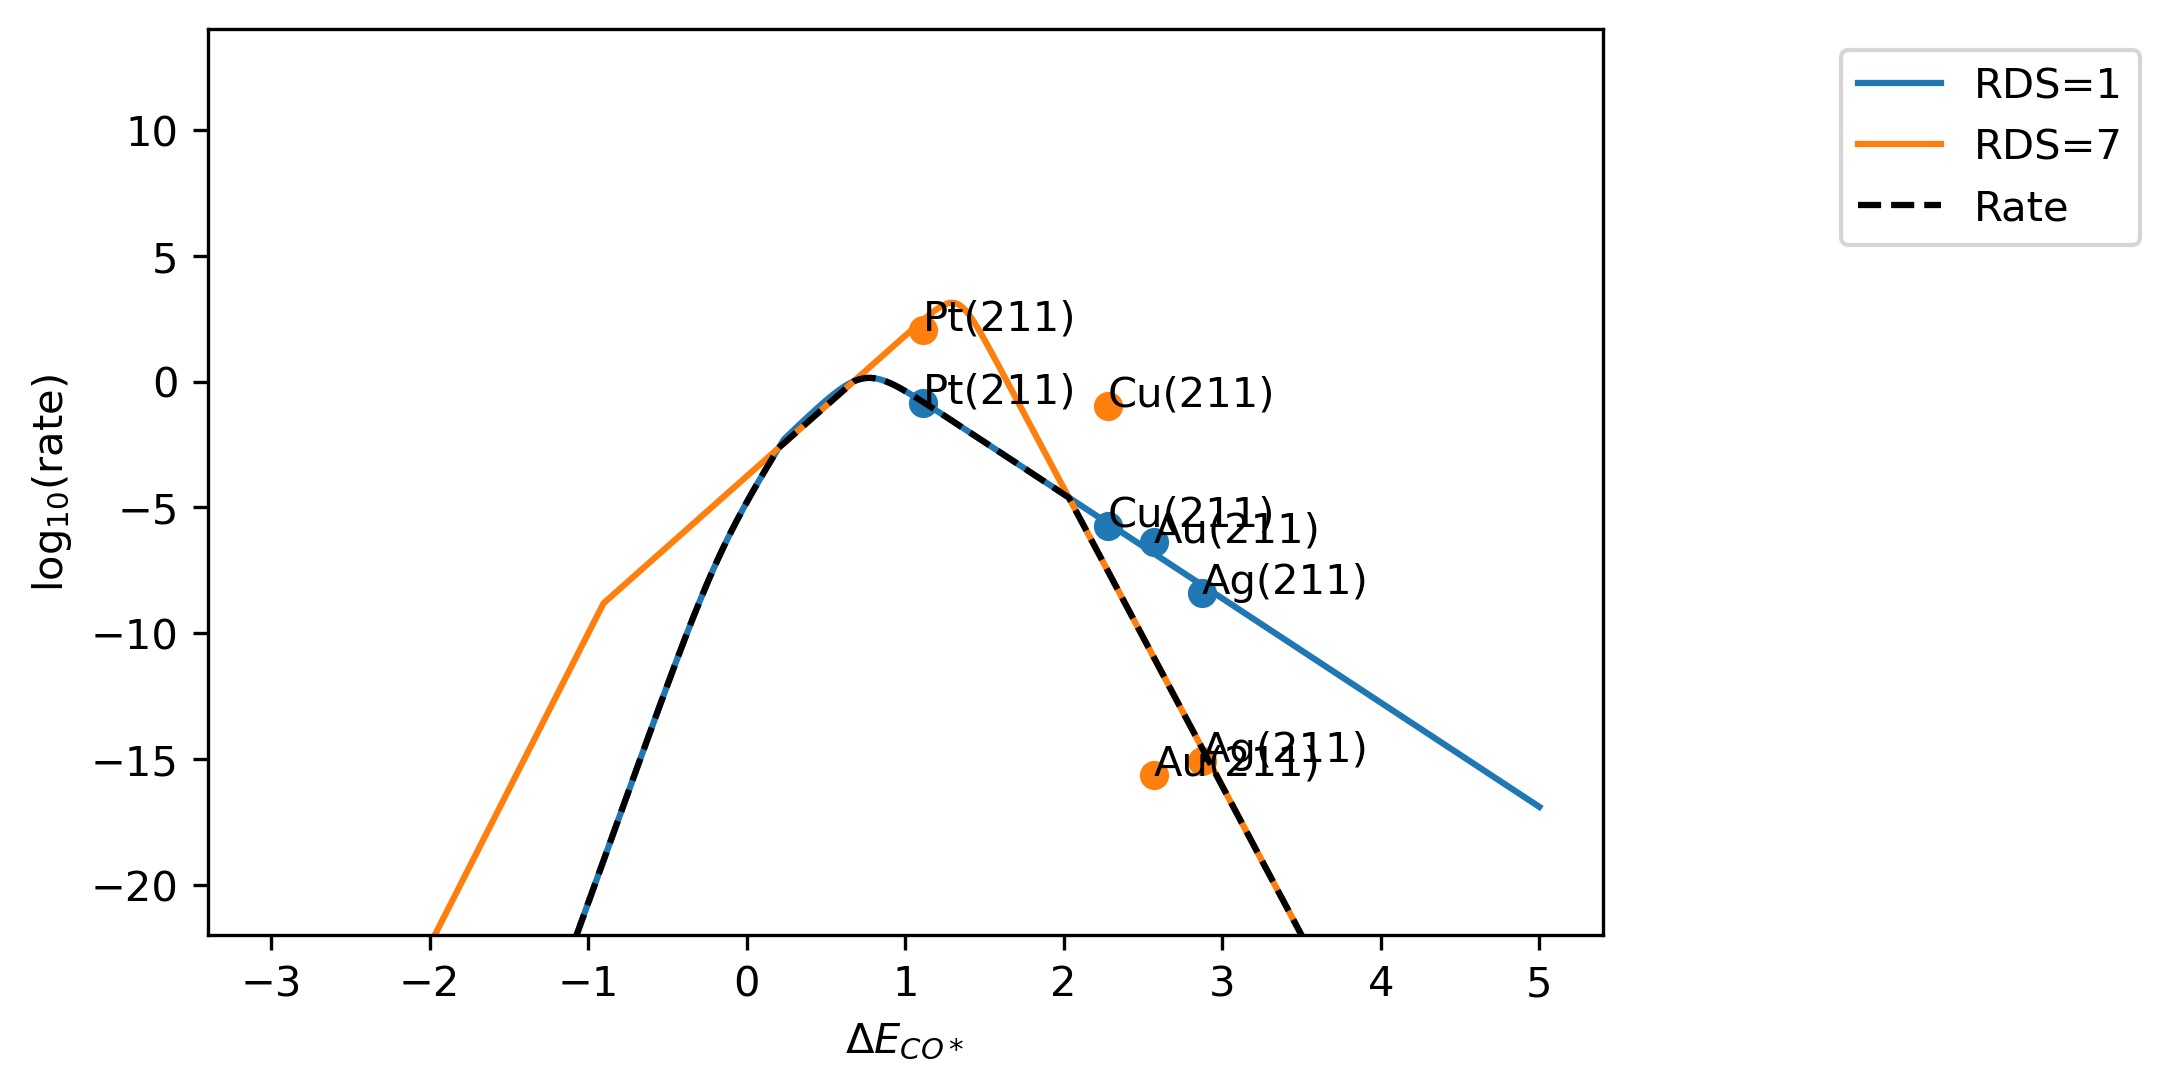
\includegraphics[width=0.8\textwidth]{Pictures/Kinetic_calculation.png}
        \caption{Kinetic activities of Ag(211), Au(211), Cu(211) and Pt(211) surfaces.}
        \label{fig:Kinetic_calculation}
    \end{figure}
    
    \subsection*{Activity volcano(s)}
    The kinetic activities of Ru(211) and Rh(211) cannot be directly calculated because their reaction energies and activation energies in step 9 are not in the database of catapp. According to the scaling relation between $\Delta E_{CO*}$ and $ \Delta E_{CH_3-H*}$, we can get $\Delta E_{CO*}$ of Ru(211) and Rh(211). ($\Delta E_{CH_3-H*} = 0.822 * \Delta E_{CO*} - 0.192$) Therefore, their kinetic activities are added in Figure \ref{fig:Activity_volcano}.
    \FloatBarrier
    \begin{figure}[!ht]
        \centering
        % \includegraphics[width=0.25\textwidth]{mesh}
        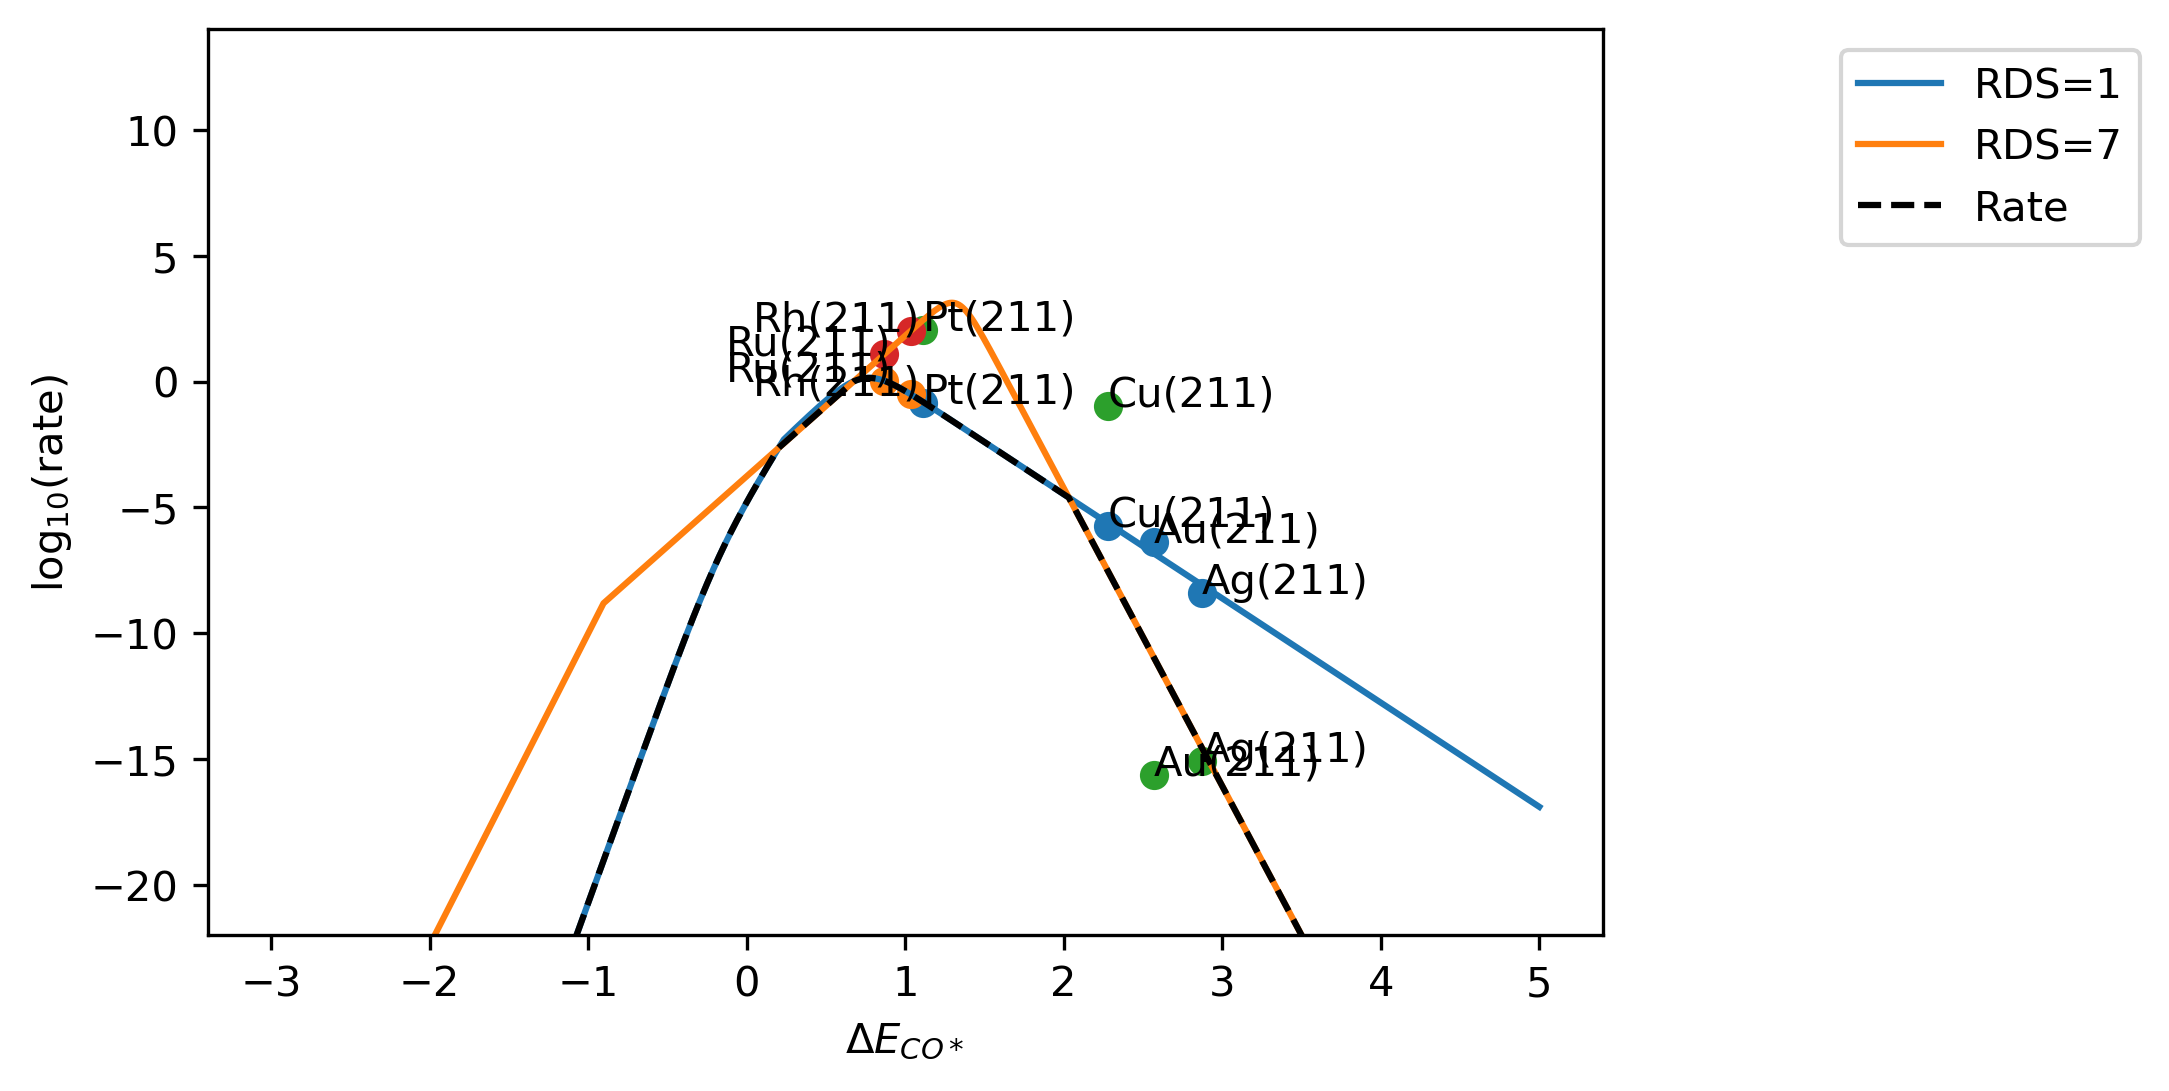
\includegraphics[width=0.8\textwidth]{Pictures/Activity_volcano.png}
        \caption{Kinetic activities of Ag(211), Au(211), Cu(211), Pt(211), Ru(211) and Rh(211) surfaces.}
        \label{fig:Activity_volcano}
    \end{figure}

    \subsection*{Discussion of electronic structure effects}
    The d-band filling of Ru(211), Rh(211), Pt(211), Cu(211), Au(211) and Ag(211) are decreasing, which are -1.41, -1.73, -2.25, -2.67, -3.56 and -4.30, respectively, according to the textbook of \textit{Fundamental concepts in heterogeneous catalysis}. Therefore, CO* binding would be weaker following this order. The best activity is around 1 eV of $\Delta E_{CO*}$ and Ru(211), Rh(211) are almost on the peak of the volcano.

\section{Discussion}
    Ru(211) and Rh(211) are almost on the peak of activity volcano, which explains why Ru and Rh have been found experimentally to be among the best materials for catalyzing this reaction. Their CO* binding neither too strong nor too weak and thus have the best catalytic performance.
\end{document}


